\section{Complexity}

\begin{definition}[\textit{Algorithm}]
    An algorithm is a step-by-step sequence of instructions designed to solve any given instance of a problem.
\end{definition}
\begin{definition}[\textit{Instance}]
    An instance, denoted as $I$, pertaining to a problem $P$, is a specific and unique case derived from the problem $P$.
\end{definition}

The runtime of an algorithm is contingent on both the specific instance and the computer it runs on. 
To assess the algorithm's complexity while abstracting from hardware variations, we focus on evaluating its performance as a function of the instance's size, independently of the underlying hardware. 
For this purpose, we consider the count of elementary operations, presuming that each operation carries an equivalent cost. 
Since determining the precise count of elementary operations is often a formidable task, we resort to considering the asymptotic count of elementary operations in the worst-case scenario.
\begin{definition}[\textit{Order of a function}]
    A function $f$ is denoted as being order of $g$ and expressed as:
    \[f(n)=O(g(n))\]
    If there exists a positive constant $c$ such that $f(n)$ is less than or equal to $c \cdot g(n)$ for sufficiently large values of $n$.
\end{definition}
We can categorize algorithms into two primary classes based on their worst-case complexity:
\begin{itemize}
    \item \textit{Polynomial}: characterized by a complexity of $O(n^d)$, where $d$ is a constant.
    \item \textit{Exponential}: demonstrating a complexity of $O(2^n)$. 
\end{itemize}
Algorithms with a high-order polynomial complexity are generally considered inefficient in practical applications.
\begin{figure}[H]
    \centering
    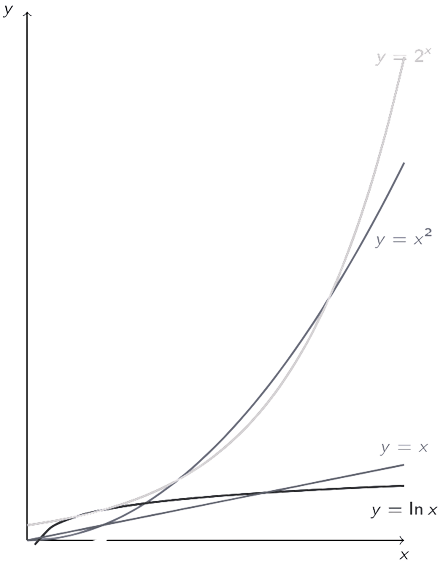
\includegraphics[width=0.5\linewidth]{images/complexity.png}
    \caption{Plot of various algorithm's complexity}
\end{figure}
\begin{definition}[\textit{Instance}]
    The size of an instance denoted as $\left\lvert I \right\rvert$ represents the number of bits required to represent that instance.
\end{definition}
\begin{definition}[\textit{Polynomially solvable}]
    A problem $P$ is considered polynomially solvable if there exists a polynomial time algorithm that can provide an optimal solution for any given instance.
\end{definition}
For many discrete optimization problems, the most efficient algorithm available today demands a number of elementary operations that, in the worst-case scenario, grows exponentially with the size of the instance.
\begin{definition}[\textit{$\mathcal{NP}$-hard}]
    $\mathcal{NP}$-hard computational problems are, at the very least, as challenging as a broad spectrum of exceptionally difficult problems for which no polynomial time algorithm has been identified to date.
\end{definition}
The $\mathcal{N}\mathcal{P}$-hardness of a problem is a very strong evidence that is inherently difficult. 
However, this doesn't imply that it cannot potentially be solved using a polynomial time algorithm.